\section{Auswertung}
\label{sec:Auswertung}
%***********************************************Auswertung a*************************
\subsection{Charakteristik des untersuchten Halogen-Zählrohrs}
Zur Untersuchung der Charakteristik des Halogen-Zählrohrs wird die gemessene Anzahl an Impulsen pro Minute auf Impulse pro Sekunde umgerechnet und gegen die angelegte Spannung aufgetragen.


\begin{longtable}{ccc}
  \caption{Messdaten zur Untersuchung der Charakteristik des Zählrohrs.}\\
  \label{tab:a}\\
\toprule
$U$/$\si{\volt}$ &$N$/$\frac{\mathrm{[Imps]}}{\si{\minute}}$&$N_\mathrm{sec}$/$\frac{\mathrm{[Imps]}}{\si{\second}}$ \\

\midrule
\endhead
\midrule
\endfoot
450 & 0 & 0,00 \\
460 & 35050 & 584,17 \\
470 & 35724 & 595,40 \\
480 & 36480 & 608,00 \\
490 & 36574 & 609,57 \\
500 & 36961 & 616,02 \\
510 & 37141 & 619,02 \\
520 & 36881 & 614,68 \\
530 & 37379 & 622,98 \\
540 & 37176 & 619,60 \\
550 & 37276 & 621,27 \\
560 & 37621 & 627,02 \\
570 & 37201 & 620,02 \\
580 & 37326 & 622,10 \\
590 & 37541 & 625,68 \\
600 & 37594 & 626,57 \\
610 & 37640 & 627,33 \\
620 & 37334 & 622,23 \\
630 & 37986 & 633,10 \\
640 & 38002 & 633,37 \\
650 & 38058 & 634,30 \\
660 & 37629 & 627,15 \\
670 & 37353 & 622,55 \\
680 & 37637 & 627,28 \\
690 & 37815 & 630,25 \\
700 & 37743 & 629,05 \\
710 & 37716 & 628,60 \\
720 & 37938 & 632,30 \\
730 & 38047 & 634,12 \\
740 & 38104 & 635,07 \\
750 & 37755 & 629,25 \\
760 & 37662 & 627,70 \\
770 & 37877 & 631,28 \\
780 & 38182 & 636,37 \\
790 & 38128 & 635,47 \\
800 & 38142 & 635,70 \\
810 & 38252 & 637,53 \\
820 & 37984 & 633,07 \\
830 & 38063 & 634,38 \\
840 & 38422 & 640,37 \\
850 & 38423 & 640,38 \\
860 & 38492 & 641,53 \\
870 & 38650 & 644,17 \\
880 & 38624 & 643,73 \\
890 & 38462 & 641,03 \\
900 & 38285 & 638,08 \\
\bottomrule
\end{longtable}


In Tabelle \ref{tab:a} finden sich die gemessenen Datentupel aus angelegter Spannung $U$ und gezählten Impulsen $N$ pro Minute. Zudem werden die hieraus berechneten Impulse pro Sekunde $N_\mathrm{sec}$ und die Breite des zugehörigen Vertrauensintervall $\sqrt{N_\mathrm{sec}}$ angegeben.\\
In Abbildung \ref{fig:a} findet sich die Zählrohrcharakteristik.
Da der Bereich der Dauerentladung mit der vorliegenden Messapparatur nicht erreicht wurde, und die Anzahl der gemessenen Impulse zum Ende der Messung wieder leicht sinkt, wird ein Fehler im Versuch angenommen und als Arbeitsbereich des Zählrohrs das Intervall von $\SI{480}{\volt}$ bis $\SI{870}{\volt}$ angenommen.
Es ergibt sich somit eine Plateaulänge von $l=\SI{390}{\volt}$.
Im Arbeitsbereich des Zählrohrs wird eine lineare Ausgleichsrechnung mit python/scipy \cite{scipy} durchgeführt.\\
Es ergeben sich die Parameter der Ausgleichgraden $y=m\cdot x+b$ zu:
\begin{align}
  m=  \num{0.061(5)}\,\frac{\mathrm{[Imps]}\cdot \si{\volt}}{\si{\second}} \text{,}\\
  b=  \num{587(4)}\,\frac{\mathrm{[Imps]}}{\si{\second}}\text{.}
\end{align}

Aus der Steigung der Ausgleichsgraden lässt sich die Steigung $P_\mathrm{S}$ im Plateaubereich zu
\begin{equation*}
  P_\mathrm{S}=\frac{\SI{6.1(5)}{\percent}}{\SI{100}{\volt}} \text{ ,}
\end{equation*}
ablesen.
\begin{figure}
  \centering
  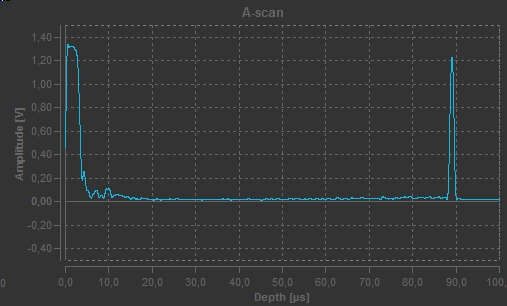
\includegraphics{Bilder/a.pdf}
  \caption{Zählrohrcharakteristik des Halogen-Zählrohrs samt markierter Plateaulänge und Ausgleichsgraden zur Bestimmung der Plateausteigung.}
  \label{fig:a}
\end{figure}
\FloatBarrier
%***********************************************




%Bild
%\begin{figure}
%  \centering
%  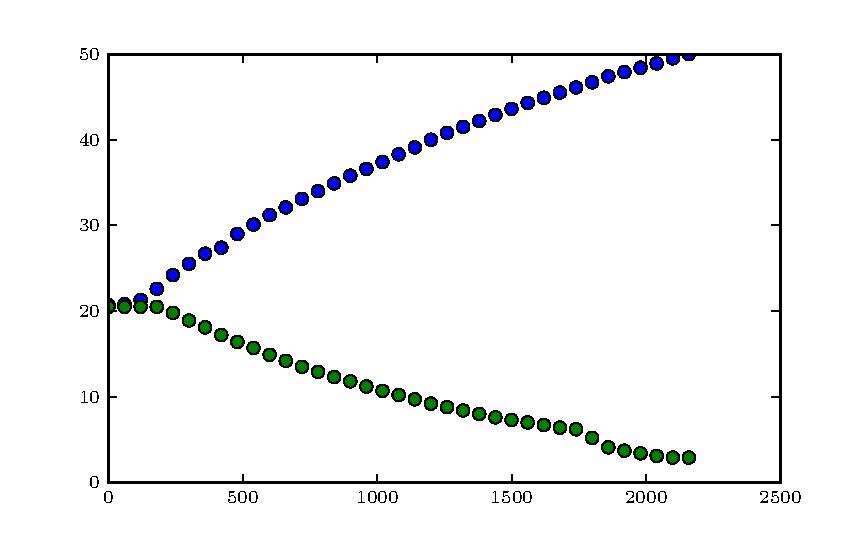
\includegraphics{plot.pdf}
%  \caption{Plot.}
%  \label{fig:plot}
%\end{figure}


%Tabelle
%\begin{table}
%	\centering
%	\caption{Table.}
%	\label{tab:table}
%	\begin{tabular}{ccc}
%		\toprule
%    column1&column2&column3\\
%		\midrule
%		220 & -391 & 659 \\
%		330 & -598 & 946 \\
%		525 & -1000 & 1660 \\
%		702 & -1337 & 2051 \\
%		930 & -1650 & 2450 \\
%		\bottomrule
%	\end{tabular}
%\end{table}
